\documentclass{article}
\usepackage{graphicx}
\usepackage{enumerate}
\usepackage{float}
\usepackage{amssymb, amsmath}
\usepackage{fancyvrb}
\usepackage{caption}
\usepackage{subcaption}
\usepackage[letterpaper, margin=1in]{geometry}


\begin{document}

\title{Assessment Report for AIA}
%\today
\author{KEE Consulting\\ 
        Los Angeles}

\maketitle
%\clearpage



\section{Data Infrastructure}

Overall the data infrastructure is in good shape. 
~\\
~\\
Greatest weakness of current dataset is that it is being populated by numerous agents each with varying standards.  This poses two problems:

\begin{itemize}
\item The accuracy of the data becomes questionable:

A bond with a ``discharged'' status may or may not have been forfeited. This makes the use of the bond status unreliable by itself.  
 
\item The variability of the data becomes unmanageable:

For data analysis to work, non-numerical data must be categorized. This allows the mathematical models to translate each category to numeric form (i.e. Male/Female $\rightarrow$ 0/1), currently:  
\begin{itemize}
\item Charges associated with bonds are filled with either state-dependent crimal codes, abreviated crime, generalizations, or left blank altogether. A suggestion would be to have drop down menu with a severity rank of crime.  
\item Defendant employement information is often filled with a business name or ``self employed'', which by itself is not very useful. A useful substitue could be an income bracket information from a drop down menu. 
\item Defendant relationships are filled with strings such as ``babby mama''. Solution would be to provide options (i.e. ex-partner).
\end{itemize}
\end{itemize}
~\\
\section{Project Roadmaps}

\subsection{Project A : \underline{A logistic regression model for Failure to Appear}}
\subsubsection{The Goal}
The goal is to construct a model which relates the probability of failure to appear (FTA) to variables through a coefficient for each variable. The Vision dataset is used jointly with the AIMS dataset. 
~\\
~\\
A regression model: A statistical analysis used to predict scores on an outcome
variable based on scores on one or more predictor variables.\\
~\\
Can be as simple as:
\begin{equation}
Y = B_{0} + B_{1}X_{1} + B_{2}X_{2} + \ldots + \epsilon_{1}+\epsilon_{2} + \ldots \\
\end{equation}
\begin{itemize}
\item Y: outcome variable (ex: Will fail to appear?)
\item X: pridictor variables (ex: Defendents age, bail amount \ldots)
\item B: coeffecients relating X's and Y
\item $\epsilon$: error terms (a.k.a residual)
\end{itemize}
~\\


\subsubsection{Validity of model}

As a proof of concept, four data variables were looked at for the initial model: \\
~\\
\textbf{Characteristic of the defendant:}
~\\ 
\begin{enumerate}
\item Age at time of the bond
\begin{figure}[H]
\centering
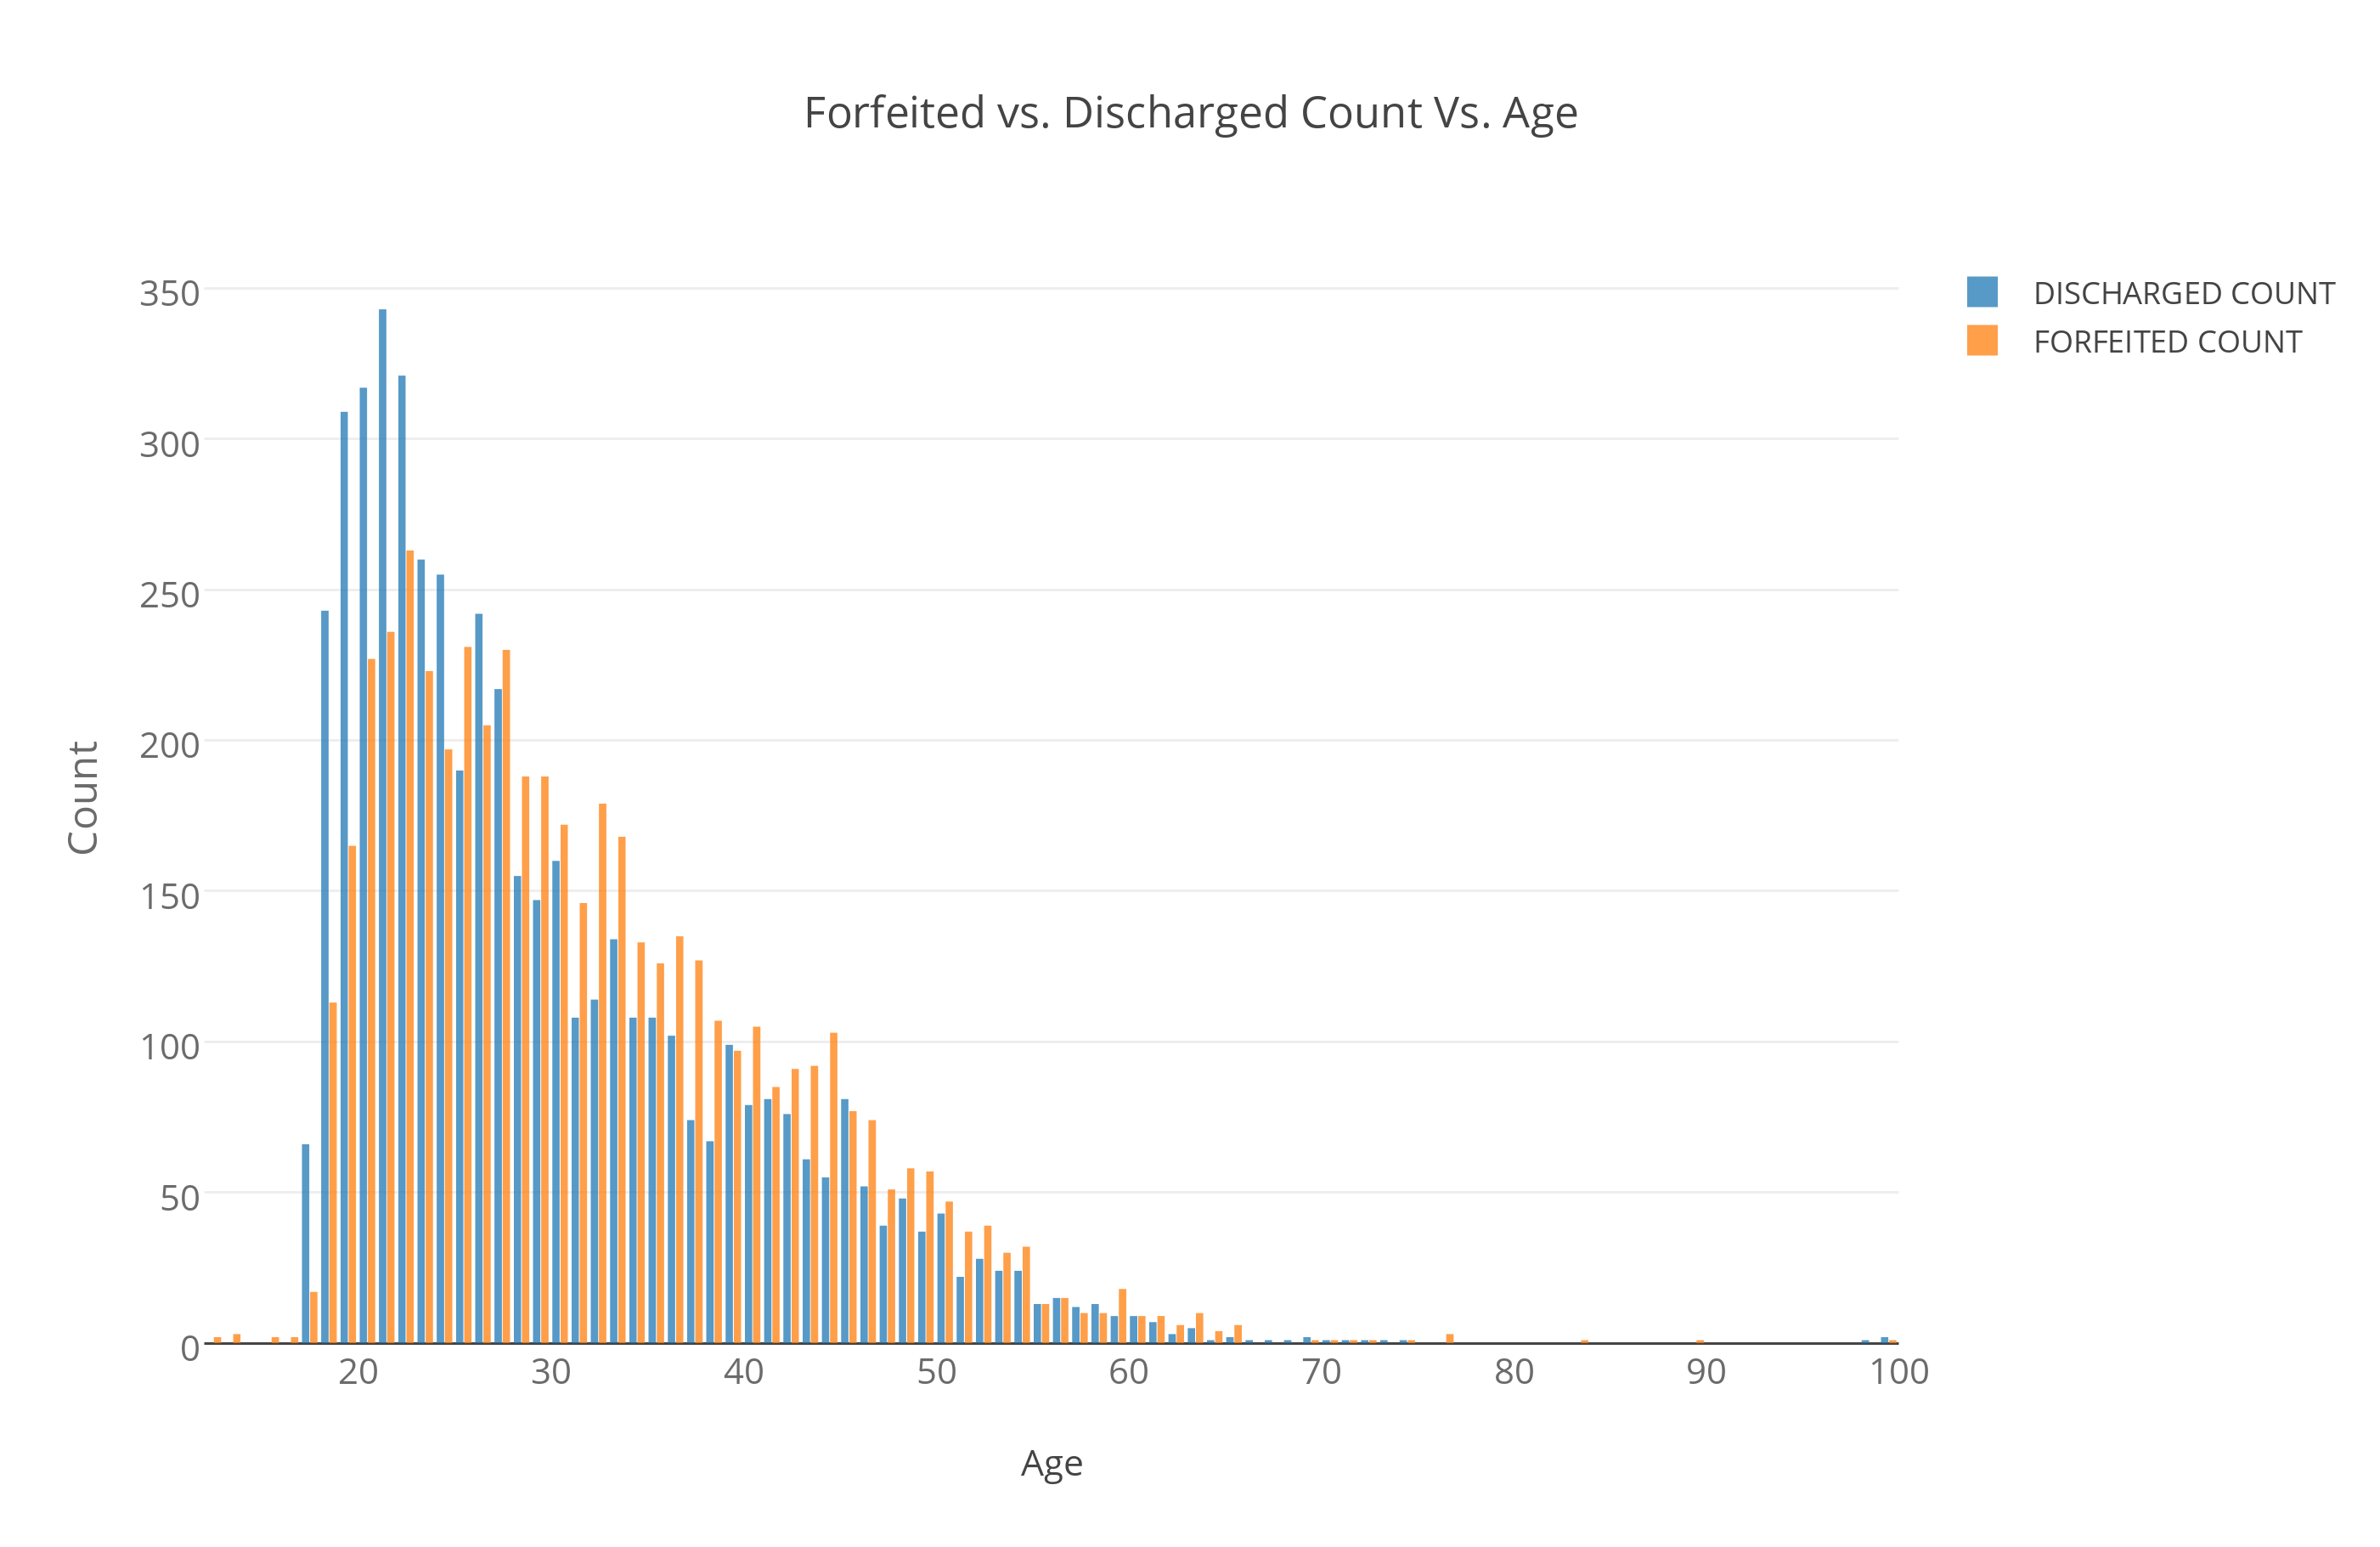
\includegraphics[width=0.5\paperwidth]{Forfeited_vs_Discharged_Count_Vs_Age.png}
\end{figure}

\item Gender
\end{enumerate}
~\\
\textbf{Characteristic of the environment:}
~\\
\begin{enumerate}
\setcounter{enumi}{2}
\item zipcode $\rightarrow$ income
\begin{figure}[H]
\centering
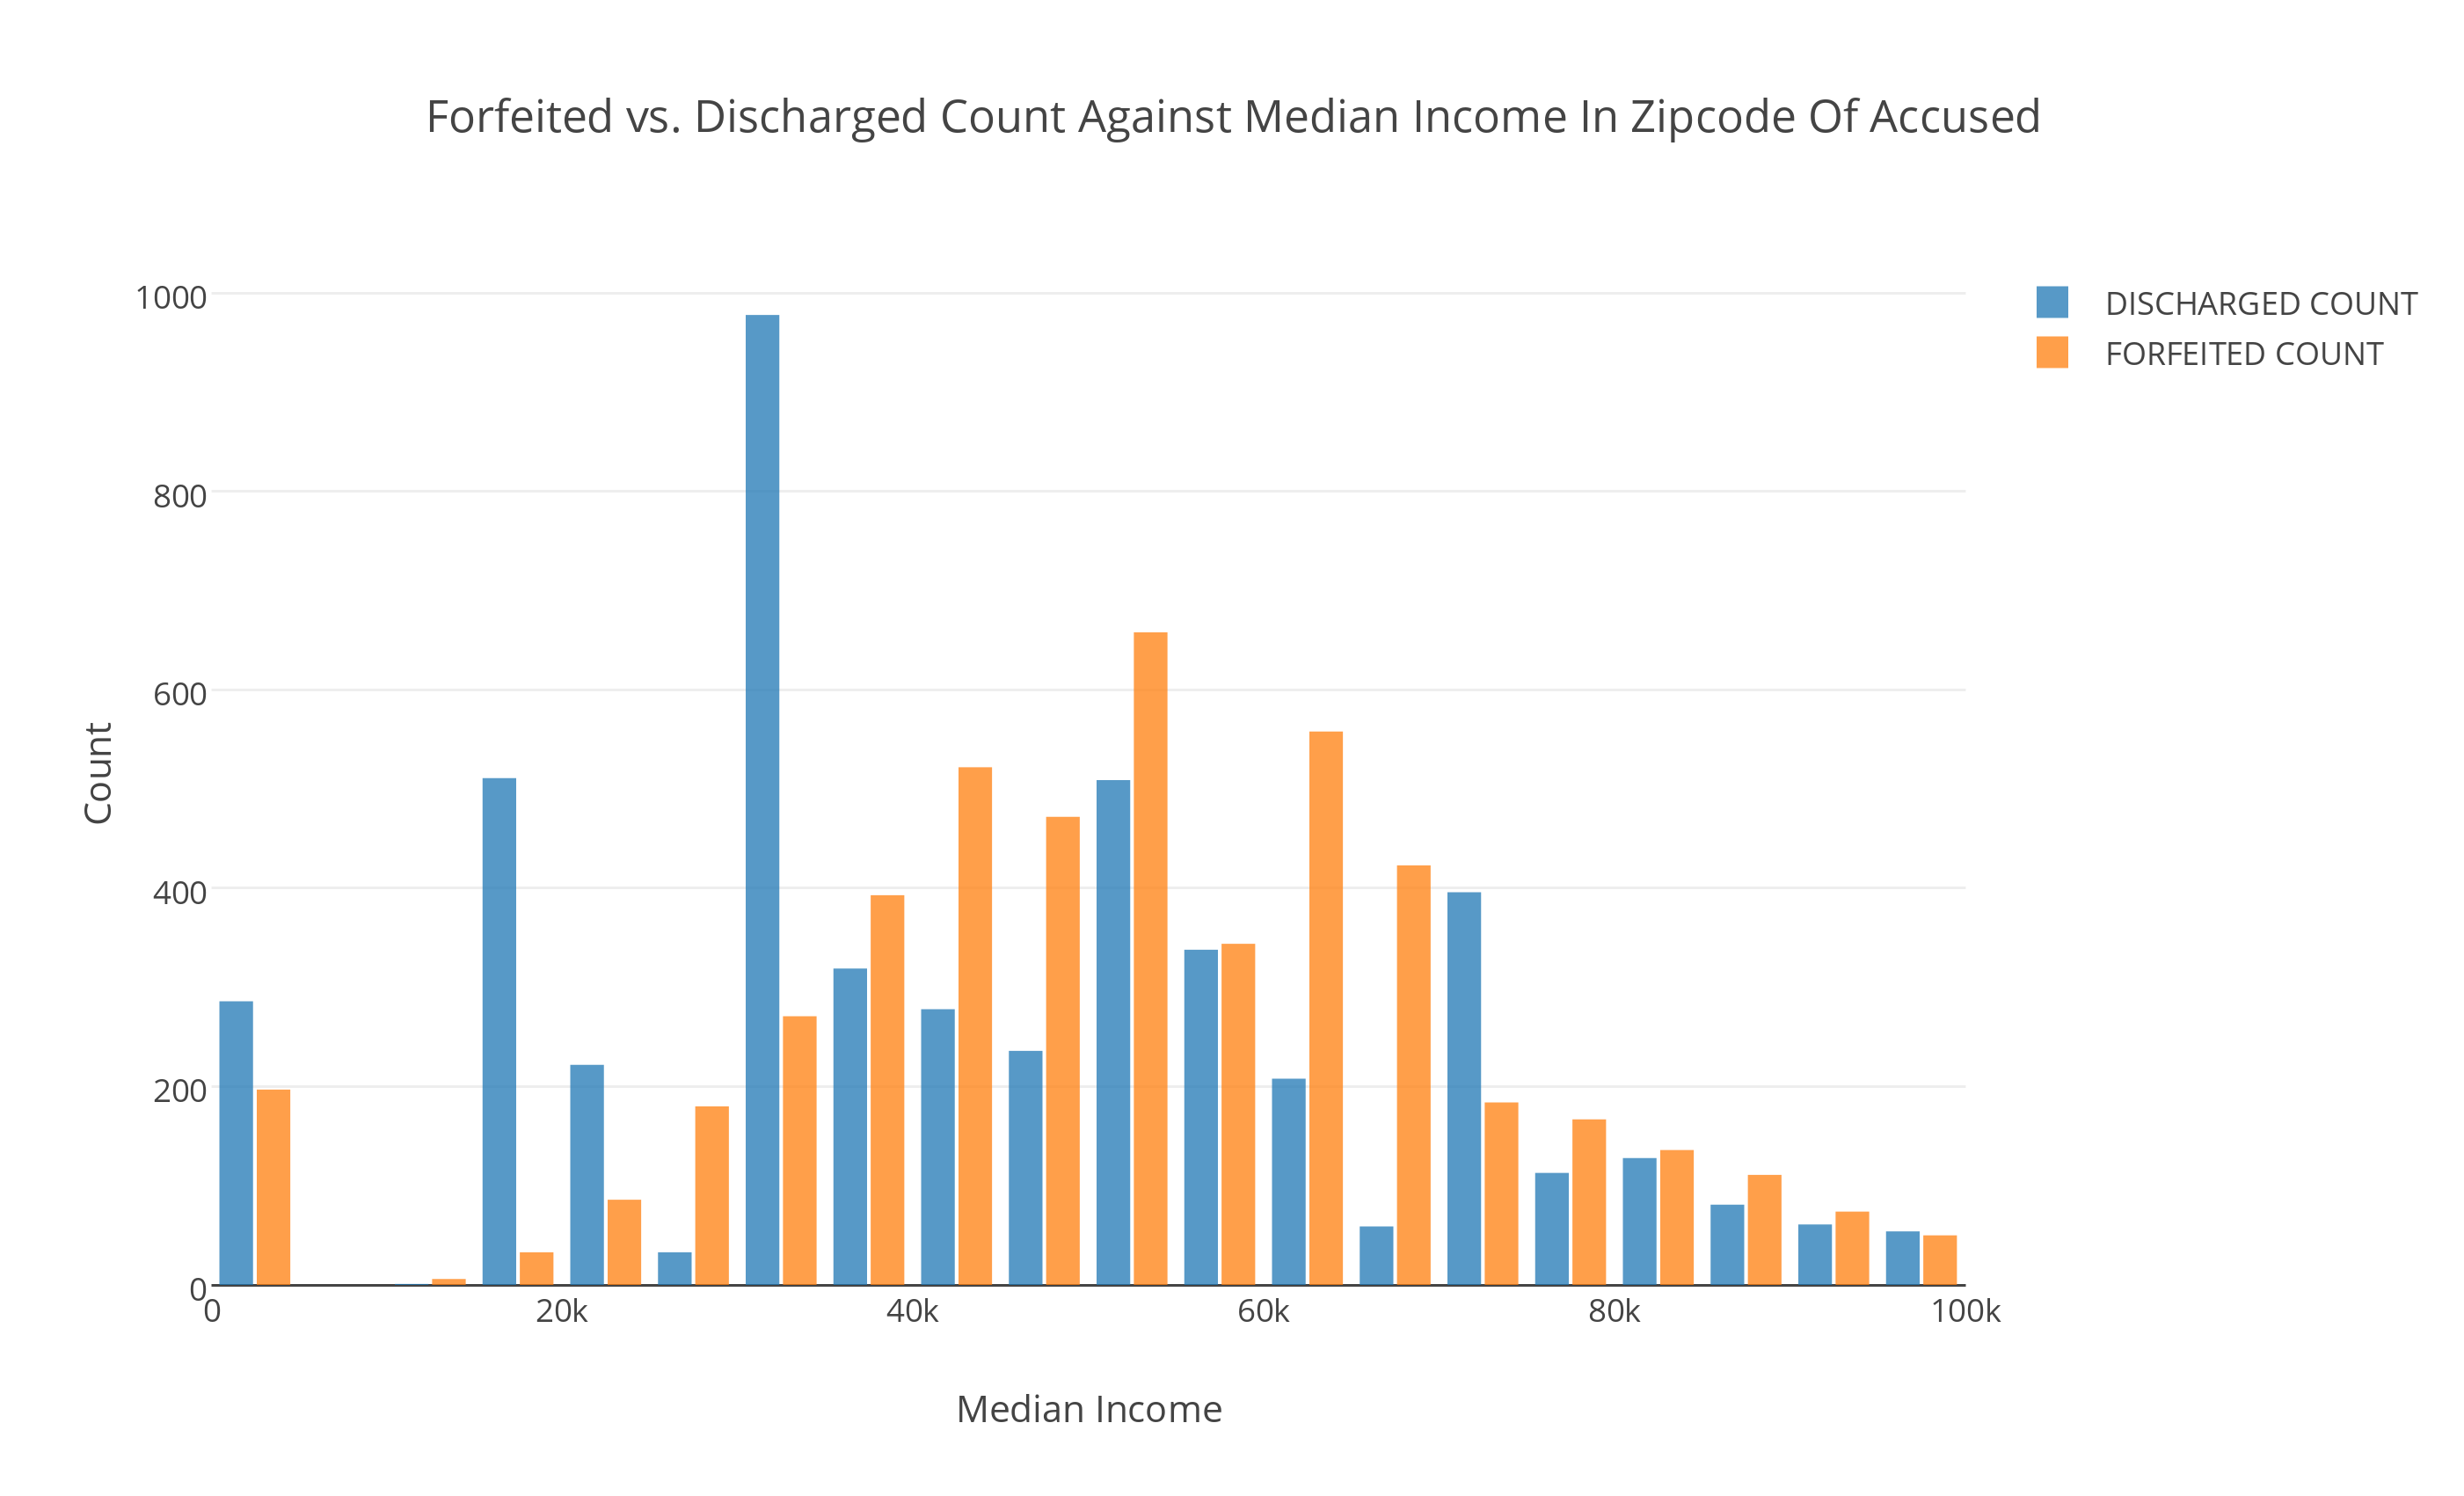
\includegraphics[width=0.5\paperwidth]{Forfeited_vs_Discharged_Count_Against_Median_Income_In_Zipcode_Of_Accused.png}
\end{figure}

The average income for a zipcode was obtained through an api to the latest available U.S. Census.   
\end{enumerate}
\textbf{Characteristic of the bond:}
~\\
\begin{enumerate}
\setcounter{enumi}{3}
\item Bond Amount
\begin{figure}[H]
\centering
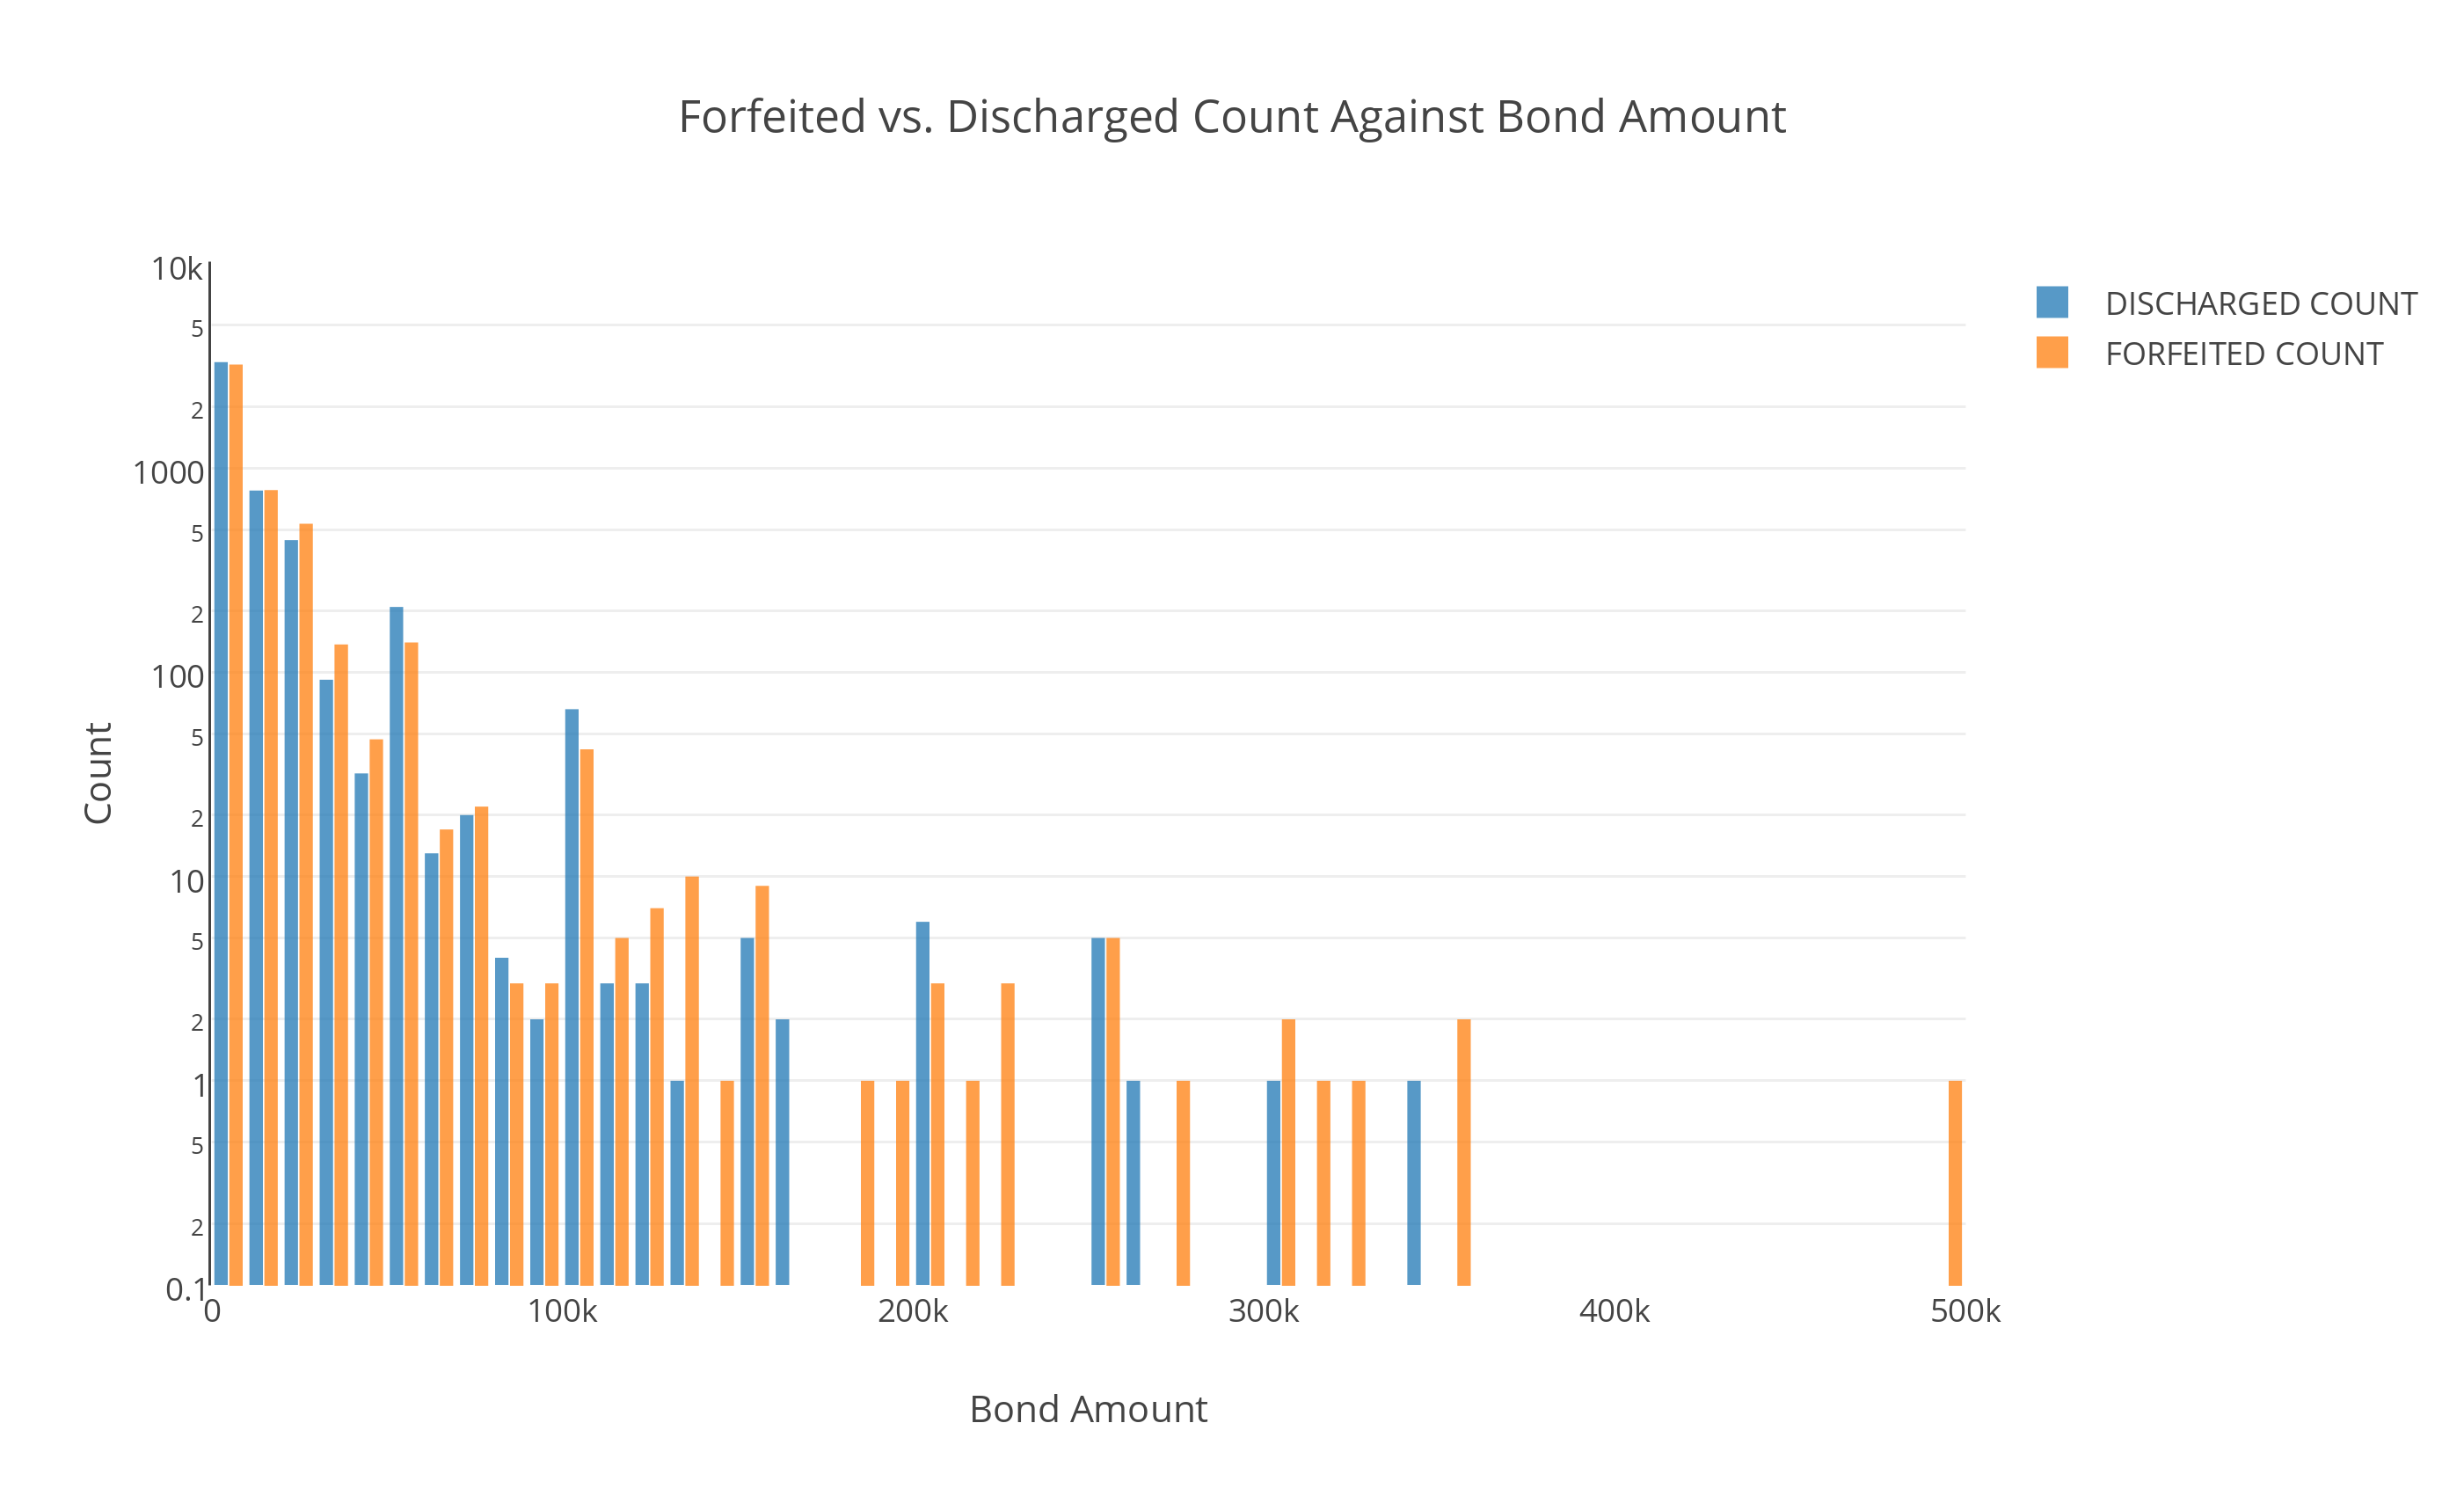
\includegraphics[width=0.5\paperwidth]{Forfeited_vs_Discharged_Count_Against_Bond_Amount.png}
\end{figure}
\end{enumerate}
~\\
\textbf{Running the Model:}
~\\
Finding a relationship between X and Y which minimizes the model errors gives us:


\begin{figure}[H]
\centering
\begin{BVerbatim}
Deviance Residuals: 
    Min       1Q   Median       3Q      Max  
-2.3472  -1.0933  -0.7349   1.1296   1.8166  

Coefficients:
                Estimate Std. Error z value Pr(>|z|)    
(Intercept)    -1.835339   0.099919 -18.368  < 2e-16 ***
catBond_Amount  0.013388   0.006470   2.069  0.03854 *  
age             0.031466   0.002381  13.213  < 2e-16 ***
catZipIncome    0.183926   0.010761  17.092  < 2e-16 ***
genderM        -0.166691   0.053297  -3.128  0.00176 ** 
---
Signif. codes:  0 ‘***’ 0.001 ‘**’ 0.01 ‘*’ 0.05 ‘.’ 0.1 ‘ ’ 1
\end{BVerbatim}
\end{figure}

%\begin{tabular}{ l | c | c }
%Variables & Defendant 1 & Defendant 2 \\
%\hline
%Age & 38  & 23 \\
%\hline
%Gender & Female & Male \\ 
%\hline
%Bond Amount & \$35,000 & \$5,000 \\ 
%\hline
%Zipcode Income & \$75,392 & \$101,905 \\
%\hline
%\hline
%calculated probablity of FTA & 75\% & 62\% \\
%& True Positve & False Positive
%\end{tabular}
%
~\\
example model predicitions:
~\\
~\\
\underline{Defendent 1:}
~\\
\begin{itemize}
\item Age: 38
\item Gender: Female 
\item Bond Amount \$35,000
\item Zipcode Income  \$75,392
\item Known to have failed to appeared
\end{itemize}
~\\
Probablity calculated by the model: 75\% to fail to appear
In reality, the bond was forfeited. This is called a ``true positive''.


~\\
\underline{Defendent 2:}
~\\
\begin{itemize}
\item Age:             23   
\item Gender:          Male
\item Bond Amount:    \$5,000
\item Zipcode Income: \$101,905
\item Known to have appeared
\end{itemize}
~\\
Probablity calculated by the model: 62\% to fail to appear
In reality, the defendant appeared in court and the bond was discharged. 
This is called a ``false positive''.
~\\
~\\
The aim is to maximize true positives and minimize false positives. 


\begin{figure}[H]
\centering
%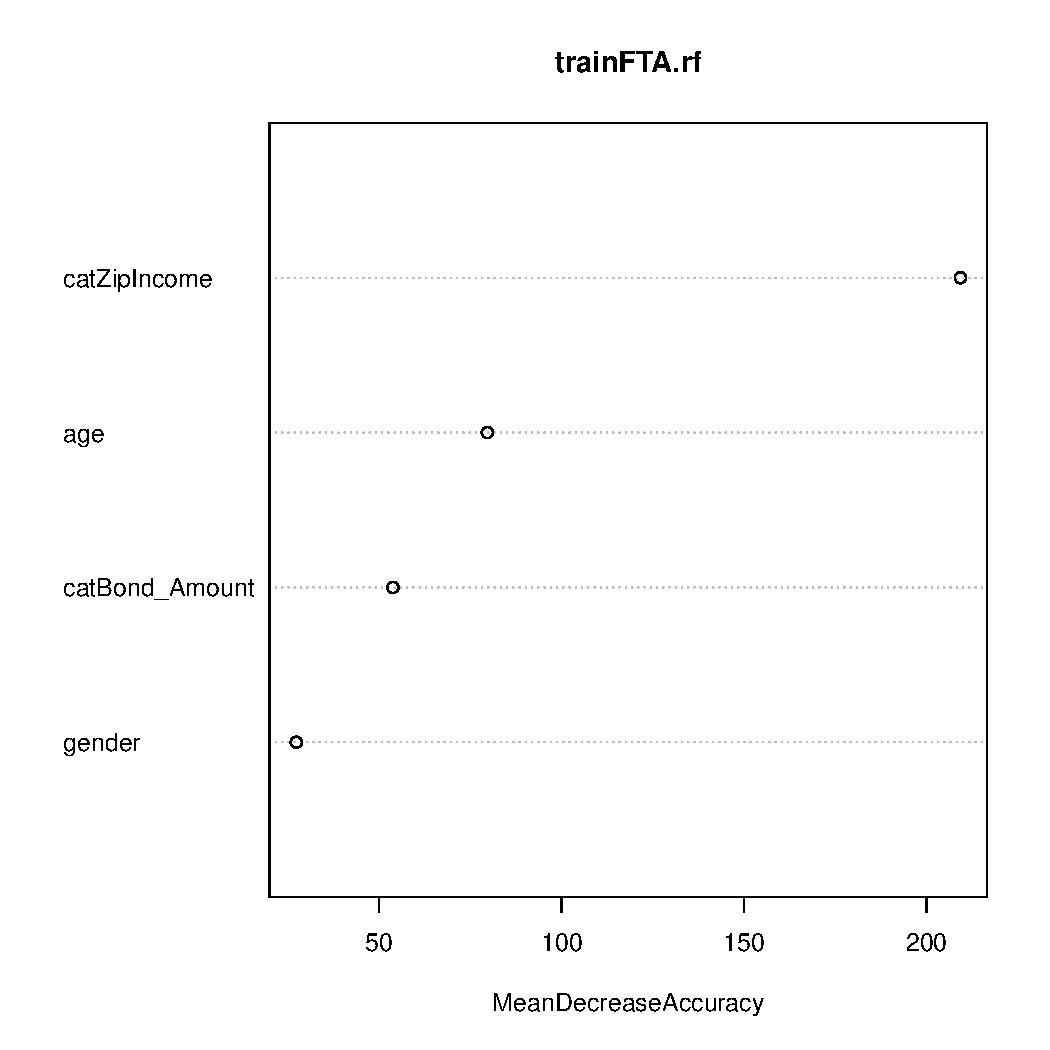
\includegraphics[width=0.45\paperwidth,page=1]{varPlot.pdf}
\includegraphics[width=0.40\paperwidth,page=3]{varPlot.pdf}
\end{figure}
 
\subsubsection{Deliverables}
A ``model'' (equation) which would allow an agent to calculate the probablity of FTA given the characteristics of the defendant and the bond.
%A confidence interval around the probability will also be calculated to give the agent a 
The validity and performance of the model will be fully tested and reported. 
   

\subsubsection{Work Estimates}
 parsing/cleaning of entire training and test datasets
 categorizing variables (ex:work/collateral/co-signers)
 constructing model
 validation of model

\textbf{1 month at \$80/hour = \$12,800}

\clearpage
\subsection{Project B: \underline{Agent Performance}}
~\\
\subsubsection{Ranking}
Ranking system: \textit{Going beyond total premimum brought in:} \\
~\\
Goal: Construct an agent ranking system to assess the ``health'' of an 
agent's business. The metric should not focus solely on the total premium 
brought in, as this unfairly compare agencies in different crime rate 
areas. The ranking metric should be built robust against fluctuations 
in premium brought in. An agent with a low penal but good ``health'' 
could indicate a bottlneck in the business.  Is the agent too 
conservative? Or is the premium rate too high? The Underwriting limit too low? Etc..
%In order to build this ranking system an initial step would be to produce performance plots of agents and AIA. Performance plots
%could include three granularities, agent level, state level, and national level: 

\begin{itemize}
\item premiums and BUF amount obtained from agents. 
\item Total penal written by agent
\item current trend
\end{itemize}

\subsubsection{The Arising Question}
Once a ranking is established  
Once the ranking metric is established, one can look for trends in the data as a solution to increase penal for an agent:
~\\
~\\
\underline{Example Question:}
\begin{center}
\begin{quote}
\textit{What contract variables contribute to premium collected? Is it Premium Rate? BUF Rate? Underwriting limit? Others?}
\end{quote}
\end{center}

~\\
Testing ``Premium Rate'':
~\\
~\\
The following figures show the premium collected from agents throughout their numerous contracts with AIA:

\begin{figure}[H]
\begin{center}
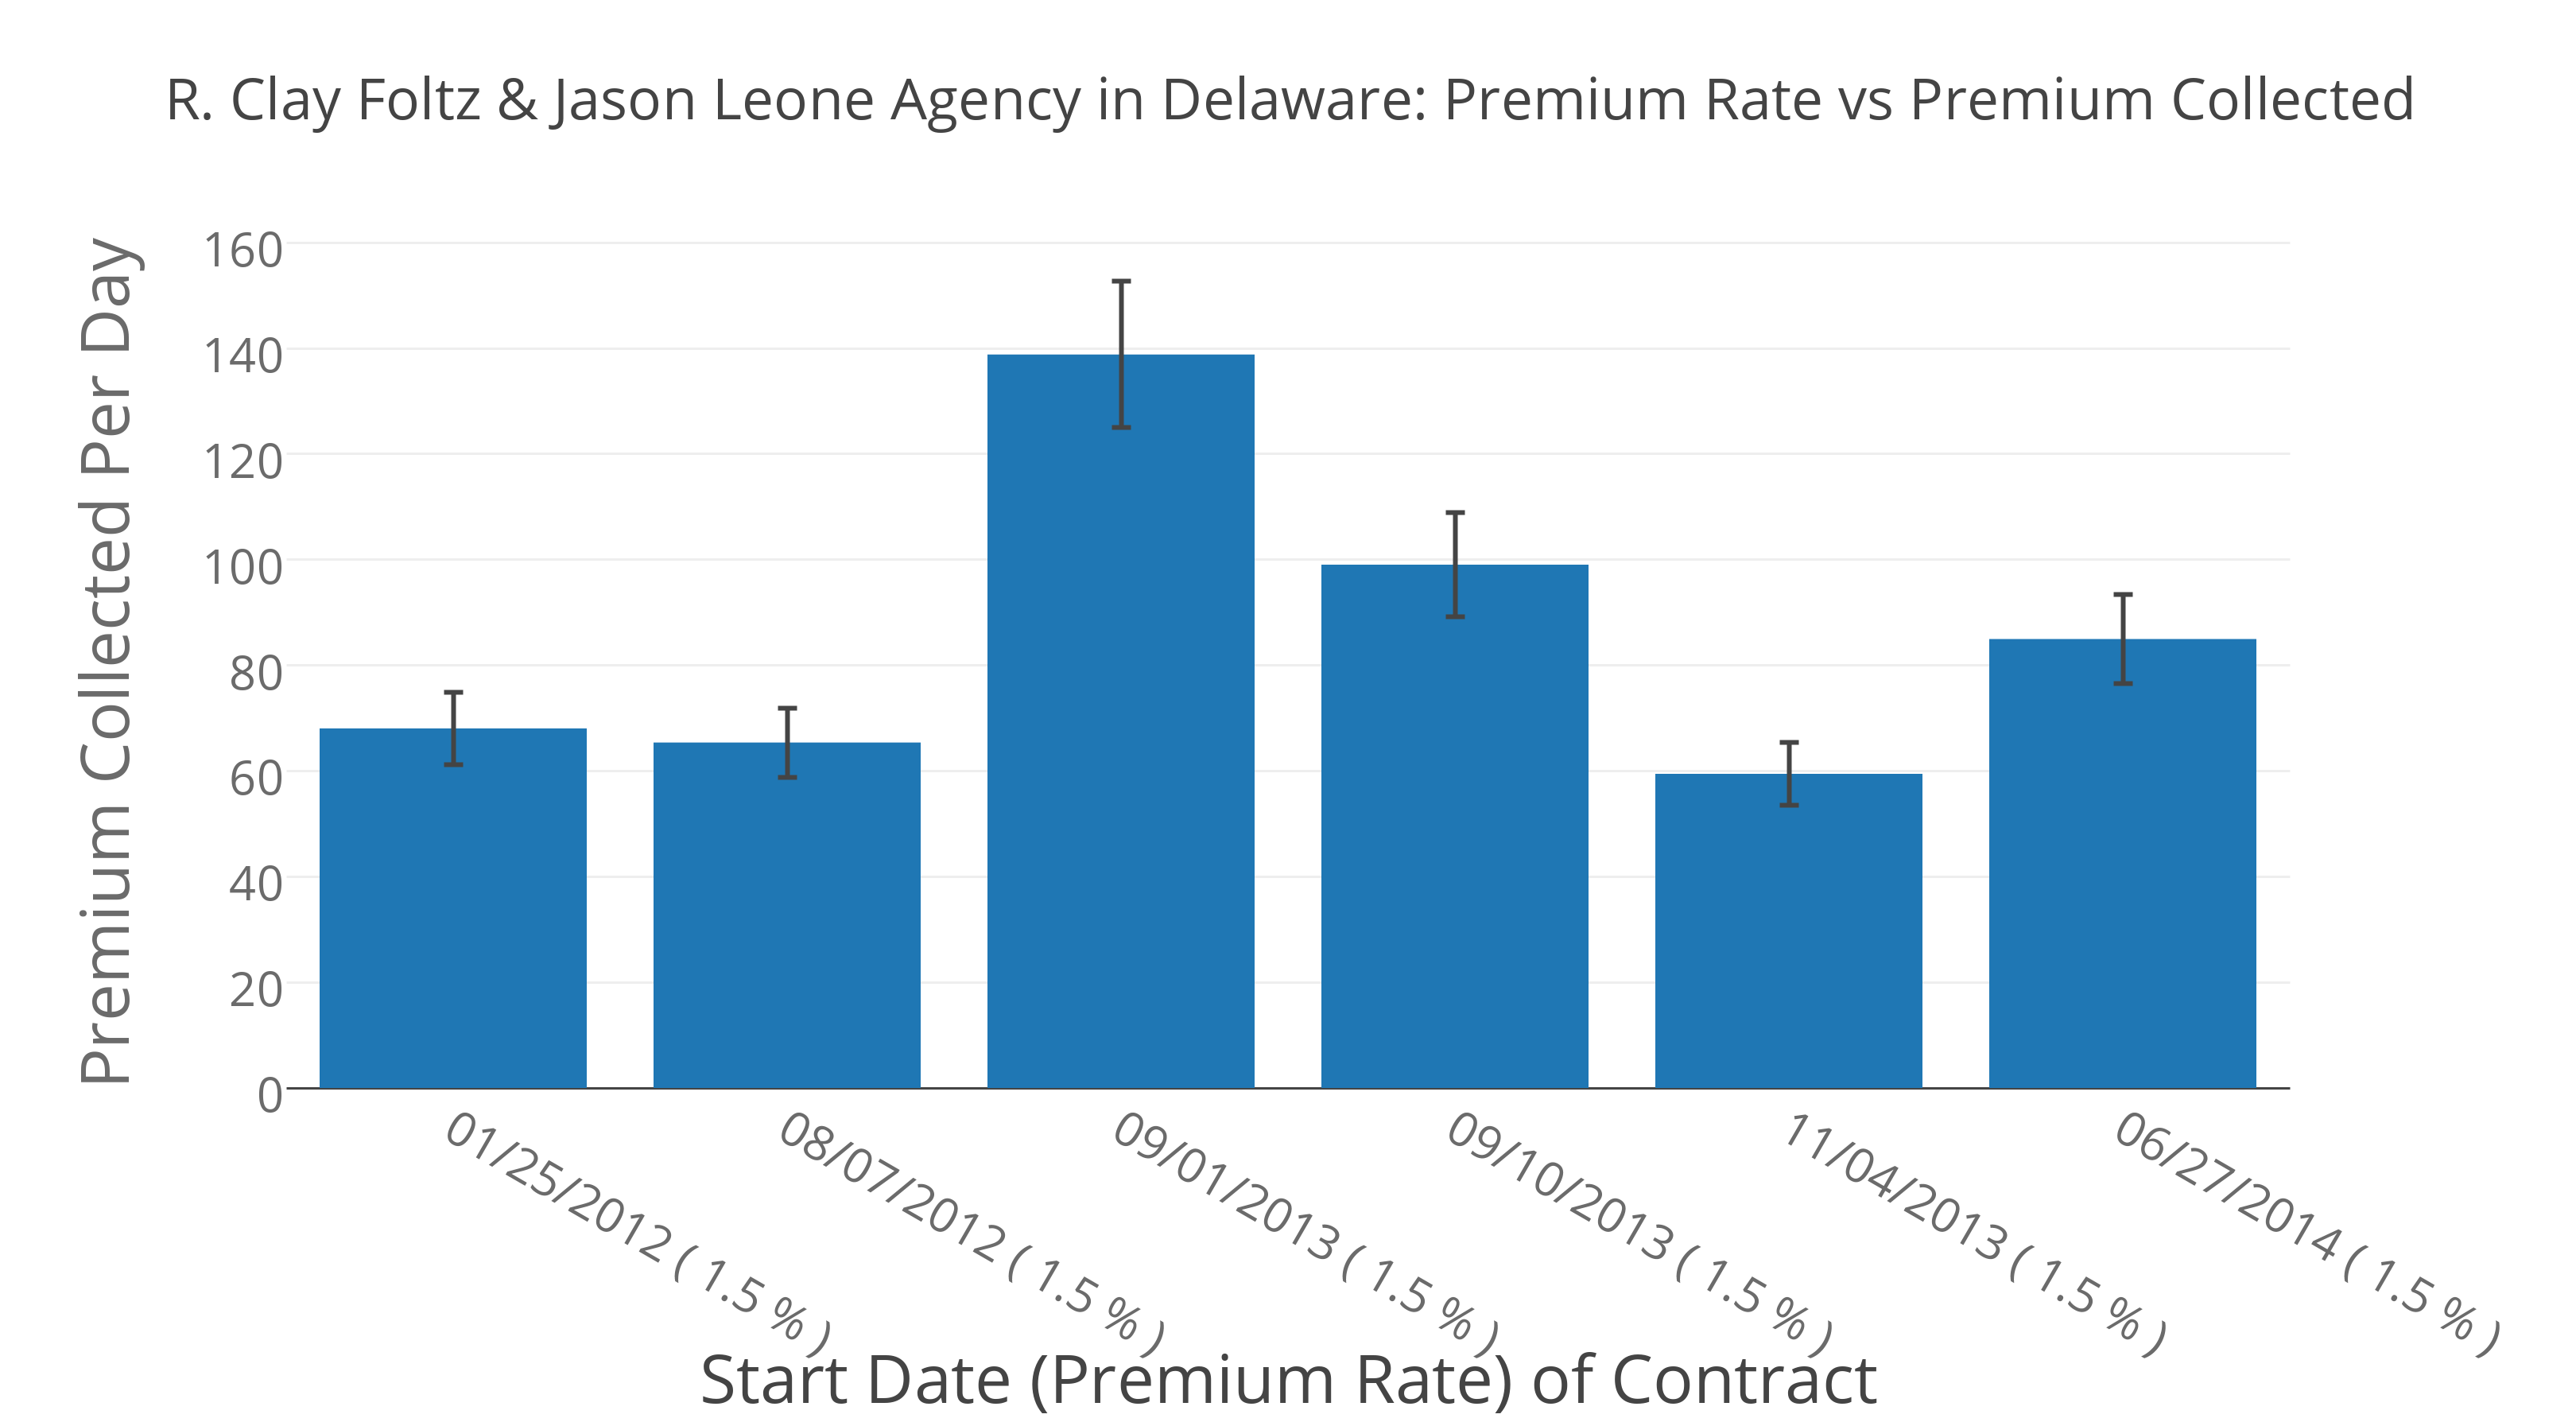
\includegraphics[width=.5\textwidth]{R_Clay_Foltz_&_Jason_Leone_Agency_in_Delaware-_Premium_Rate_vs_Premium_Collected.png}\\
\caption{An agent with a constant premium rate}
\end{center}
\end{figure}

\begin{center}
\begin{figure}[H]
\begin{subfigure}[b]{0.5\textwidth}
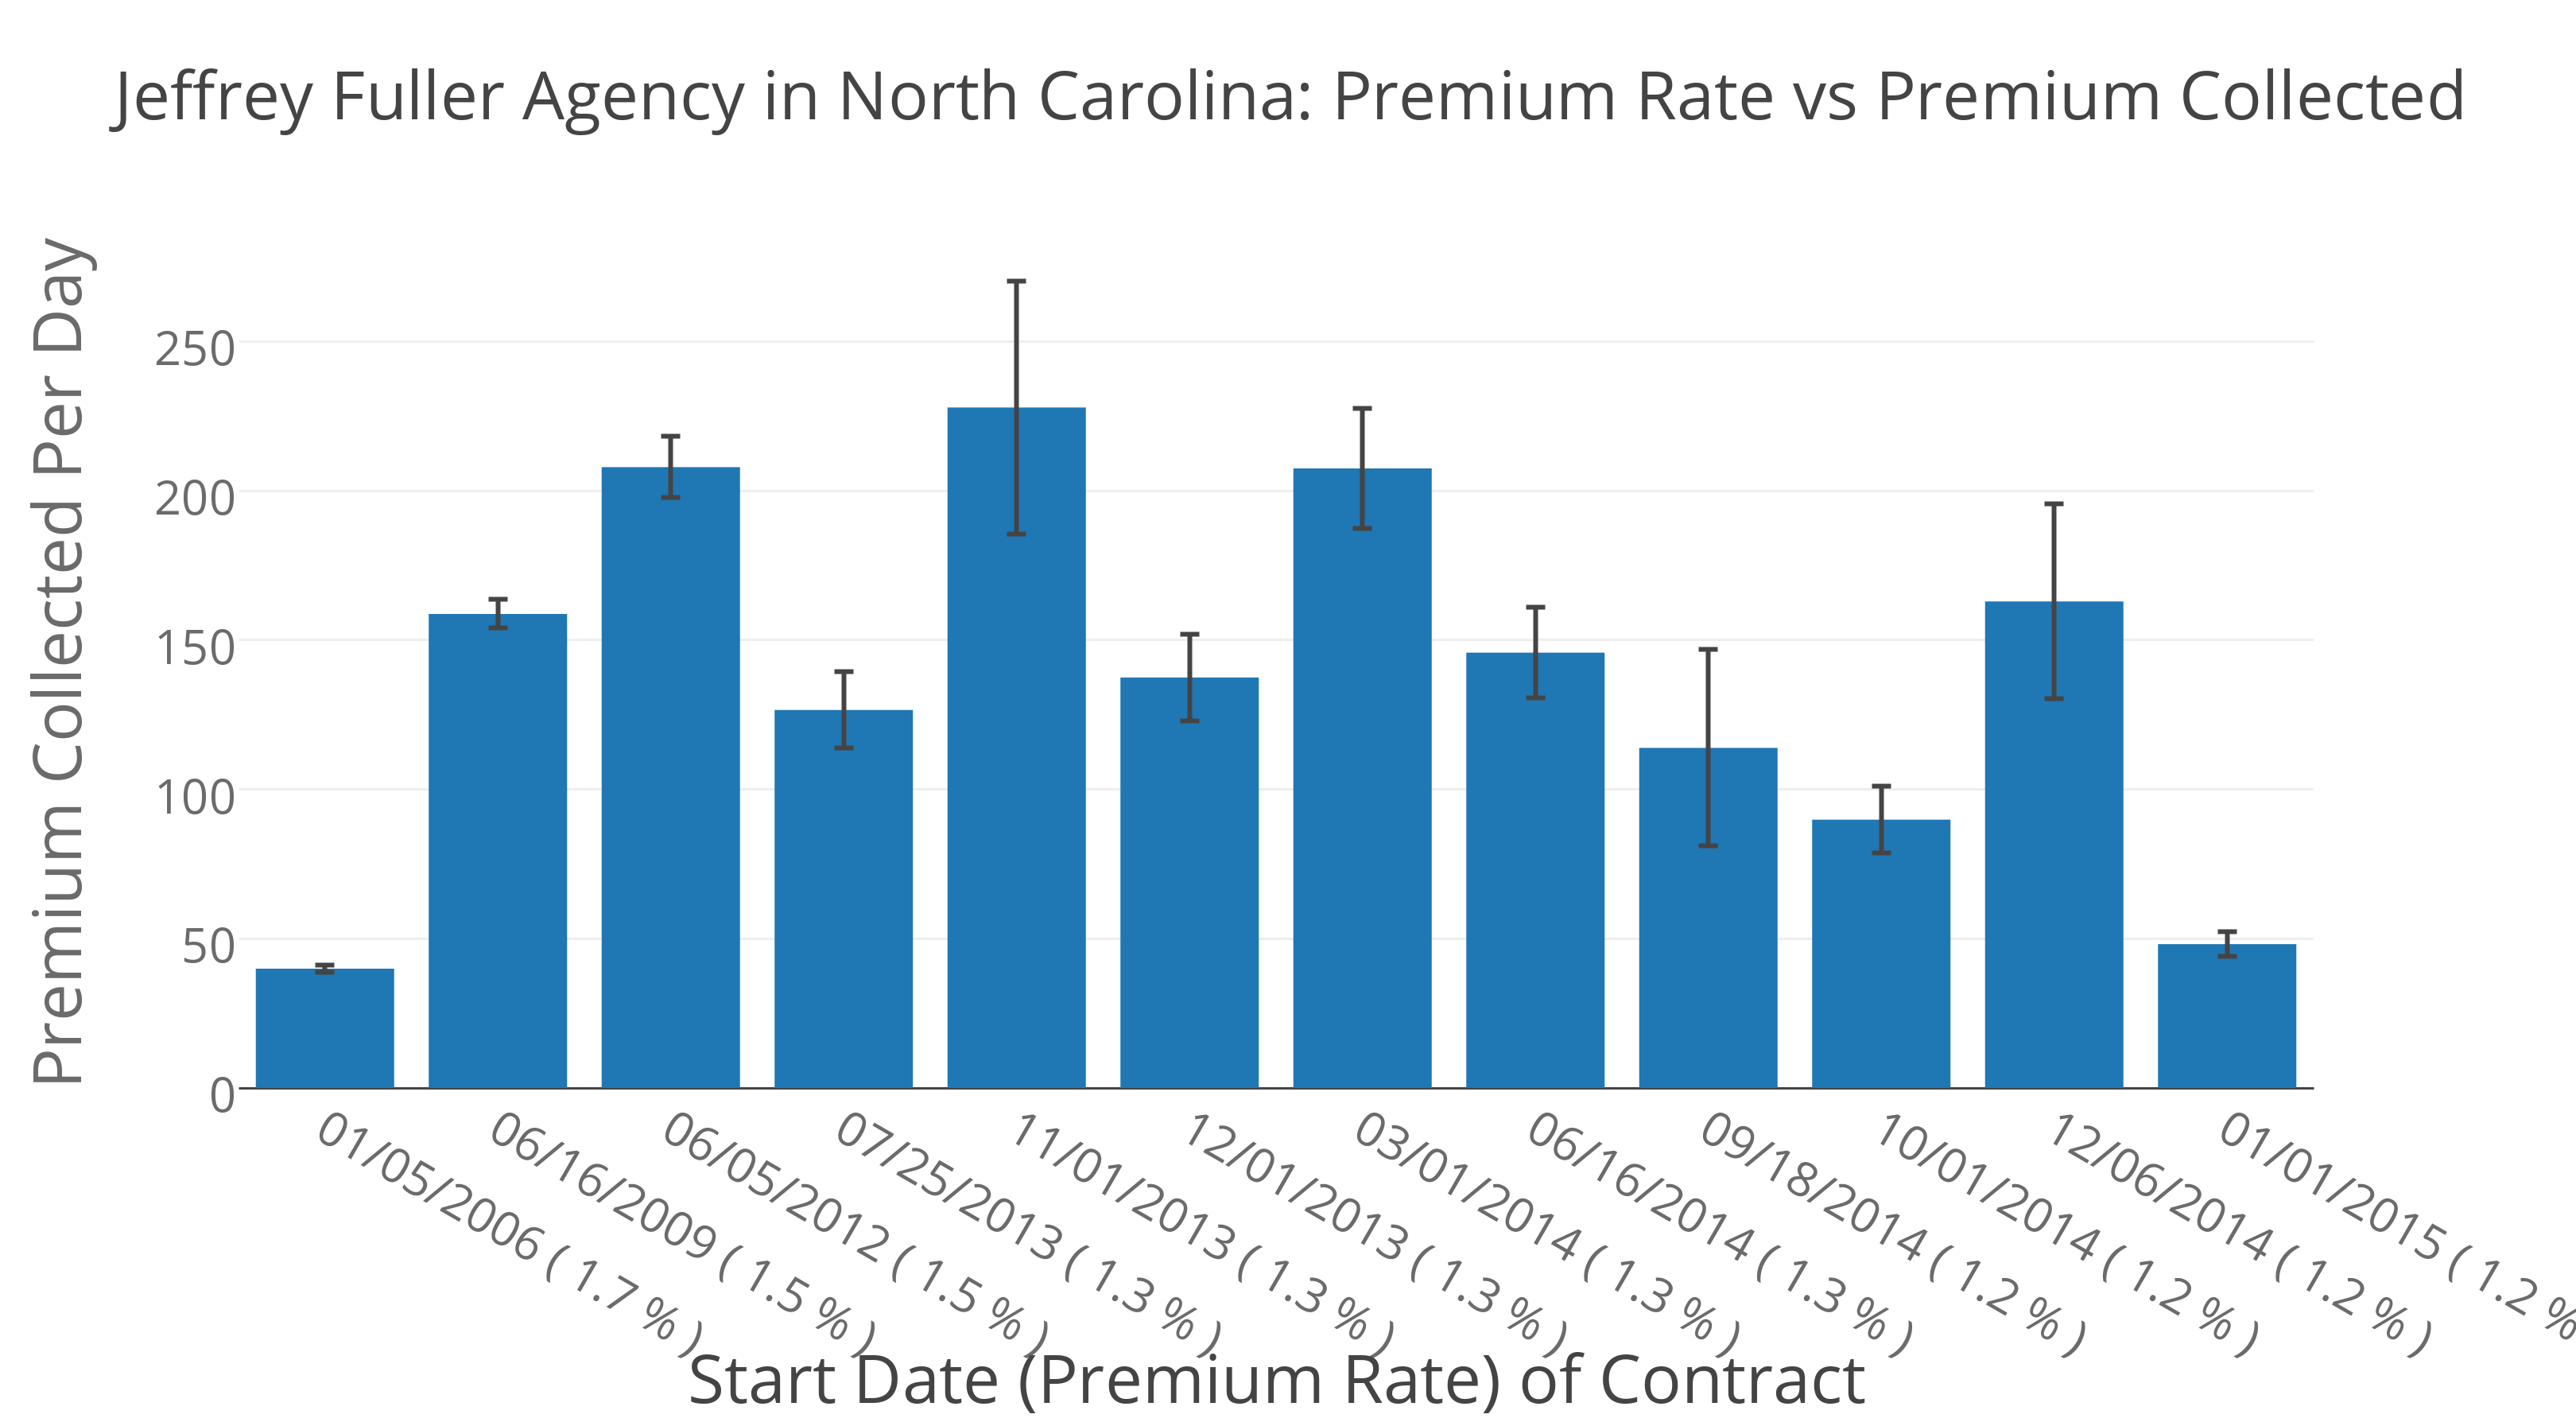
\includegraphics[width=\textwidth]{Jeffrey_Fuller_Agency_in_North_Carolina-_Premium_Rate_vs_Premium_Collected.png}
\end{subfigure}
\begin{subfigure}[b]{0.5\textwidth}
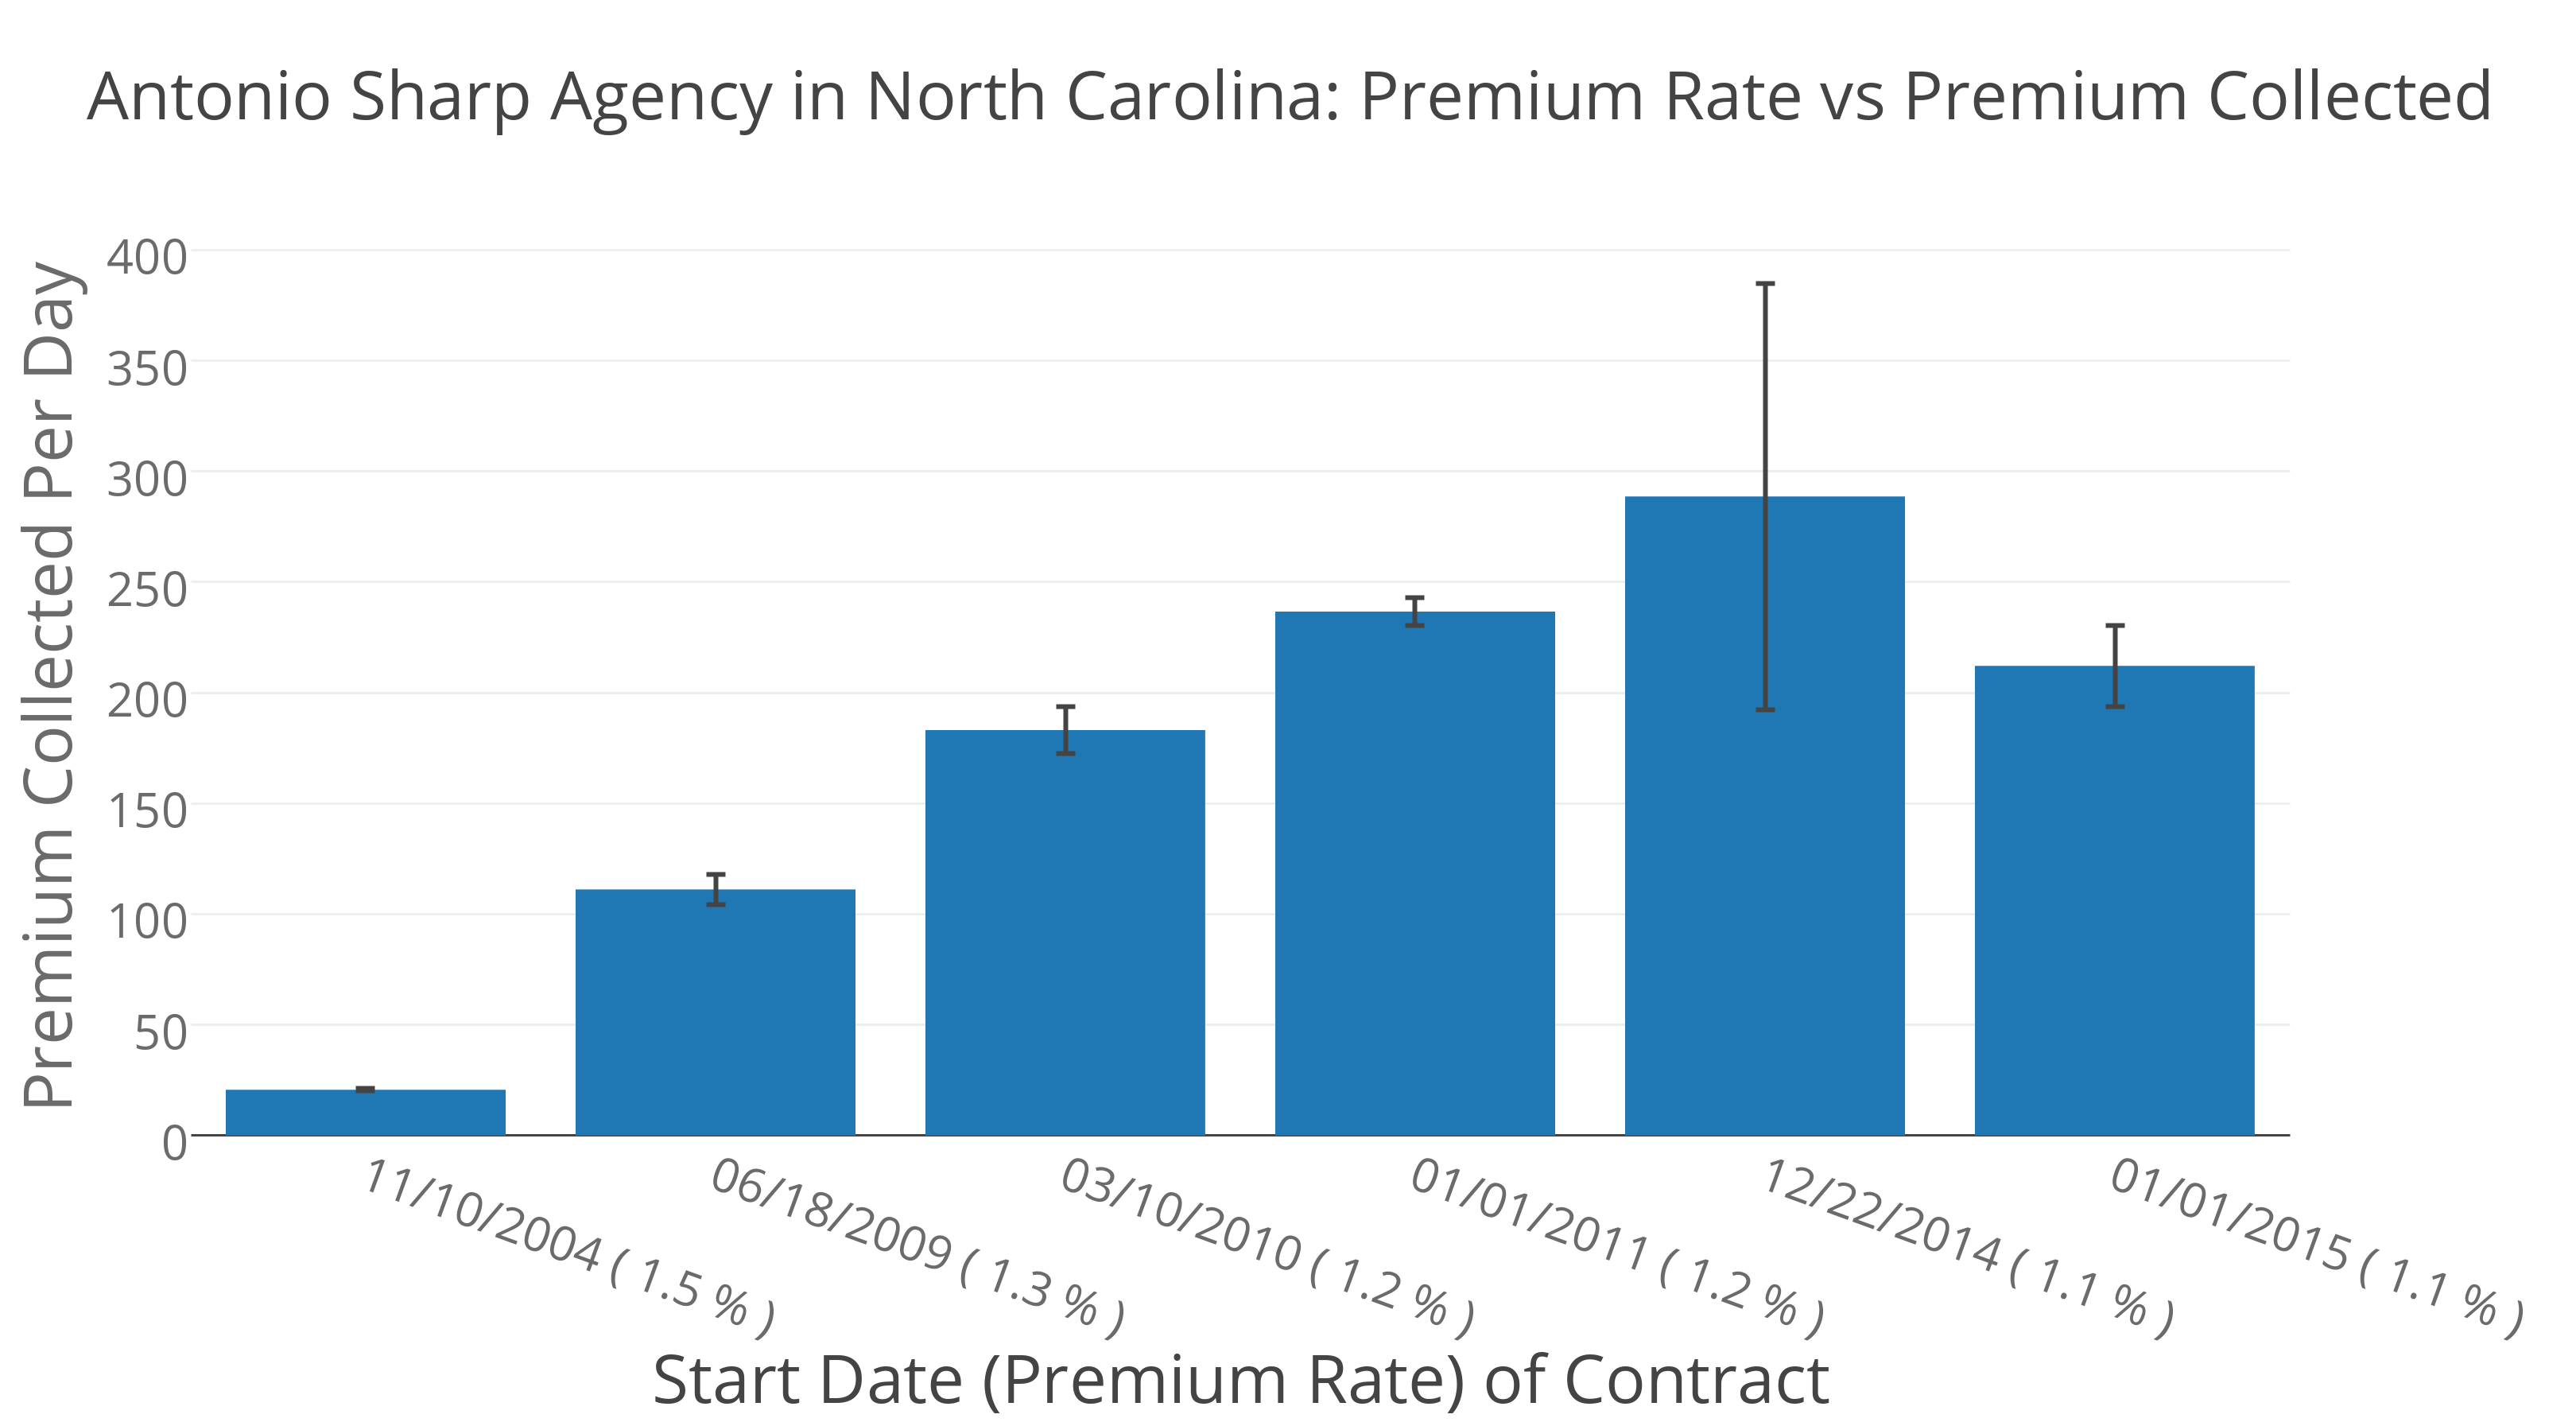
\includegraphics[width=\textwidth]{Antonio_Sharp_Agency_in_North_Carolina-_Premium_Rate_vs_Premium_Collected.png}
\end{subfigure}
\begin{subfigure}[b]{0.5\textwidth}
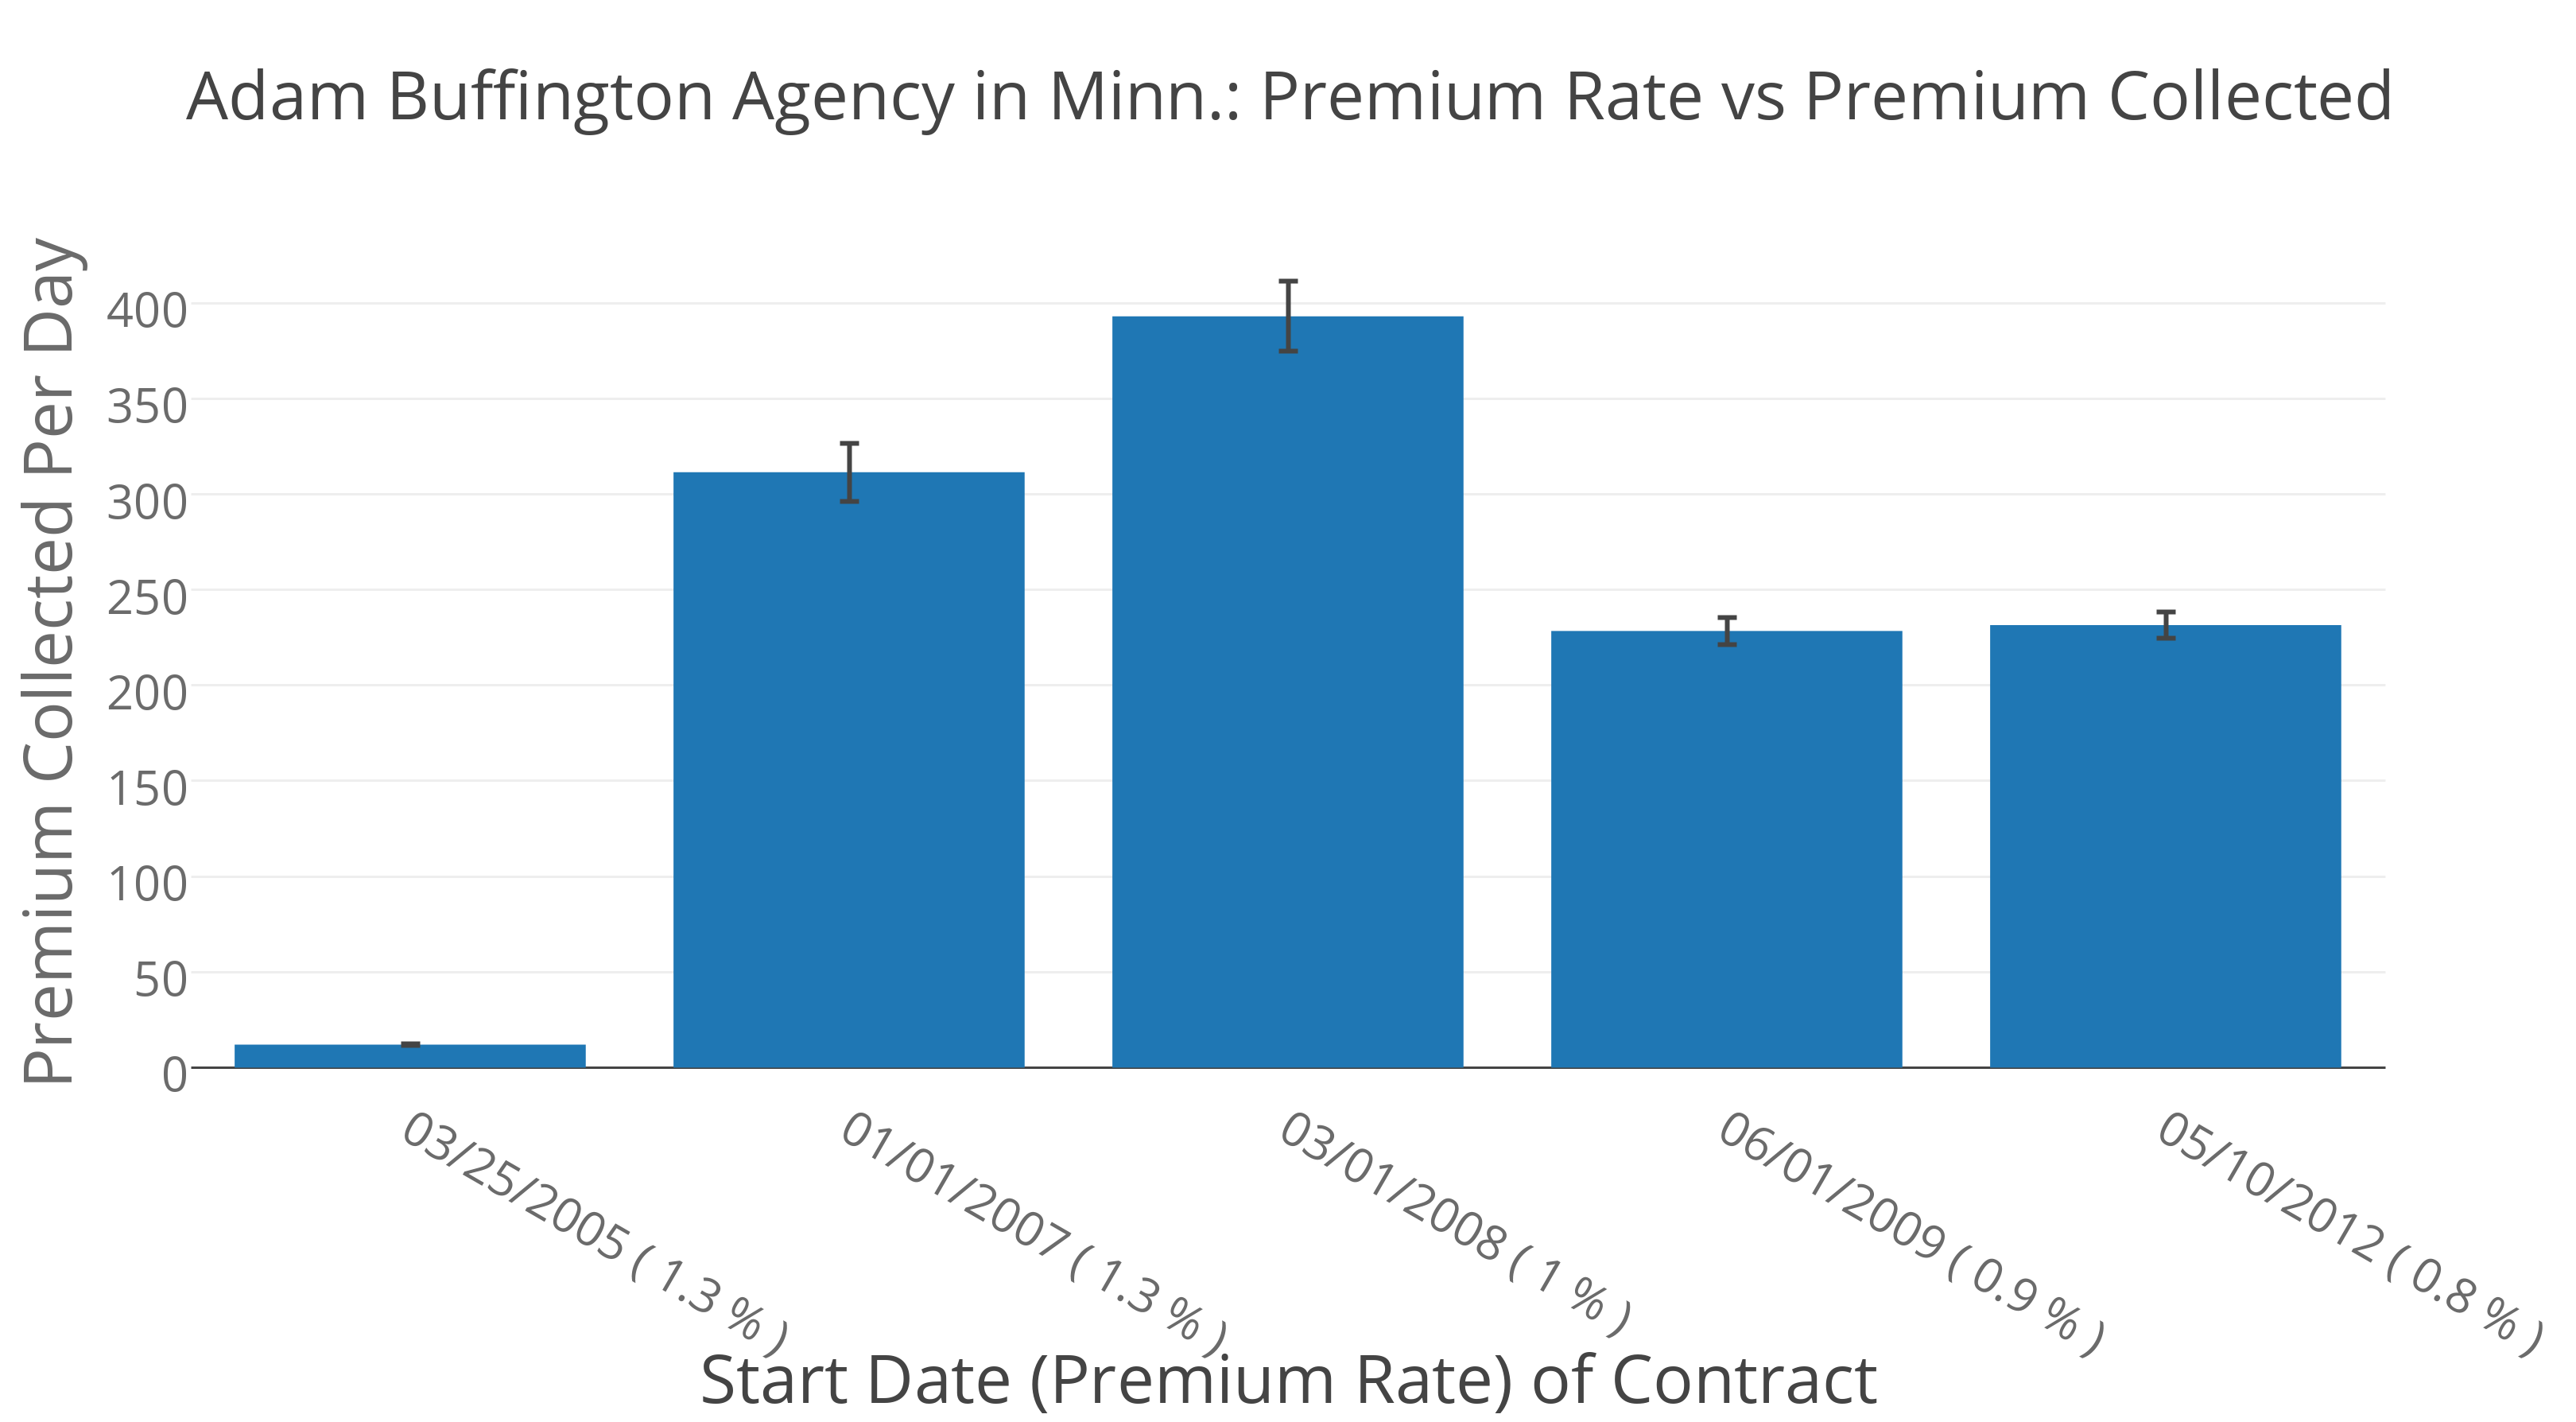
\includegraphics[width=\textwidth]{Adam_Buffington_Agency_in_Minn-_Premium_Rate_vs_Premium_Collected.png}
\end{subfigure}
\begin{subfigure}[b]{0.5\textwidth}
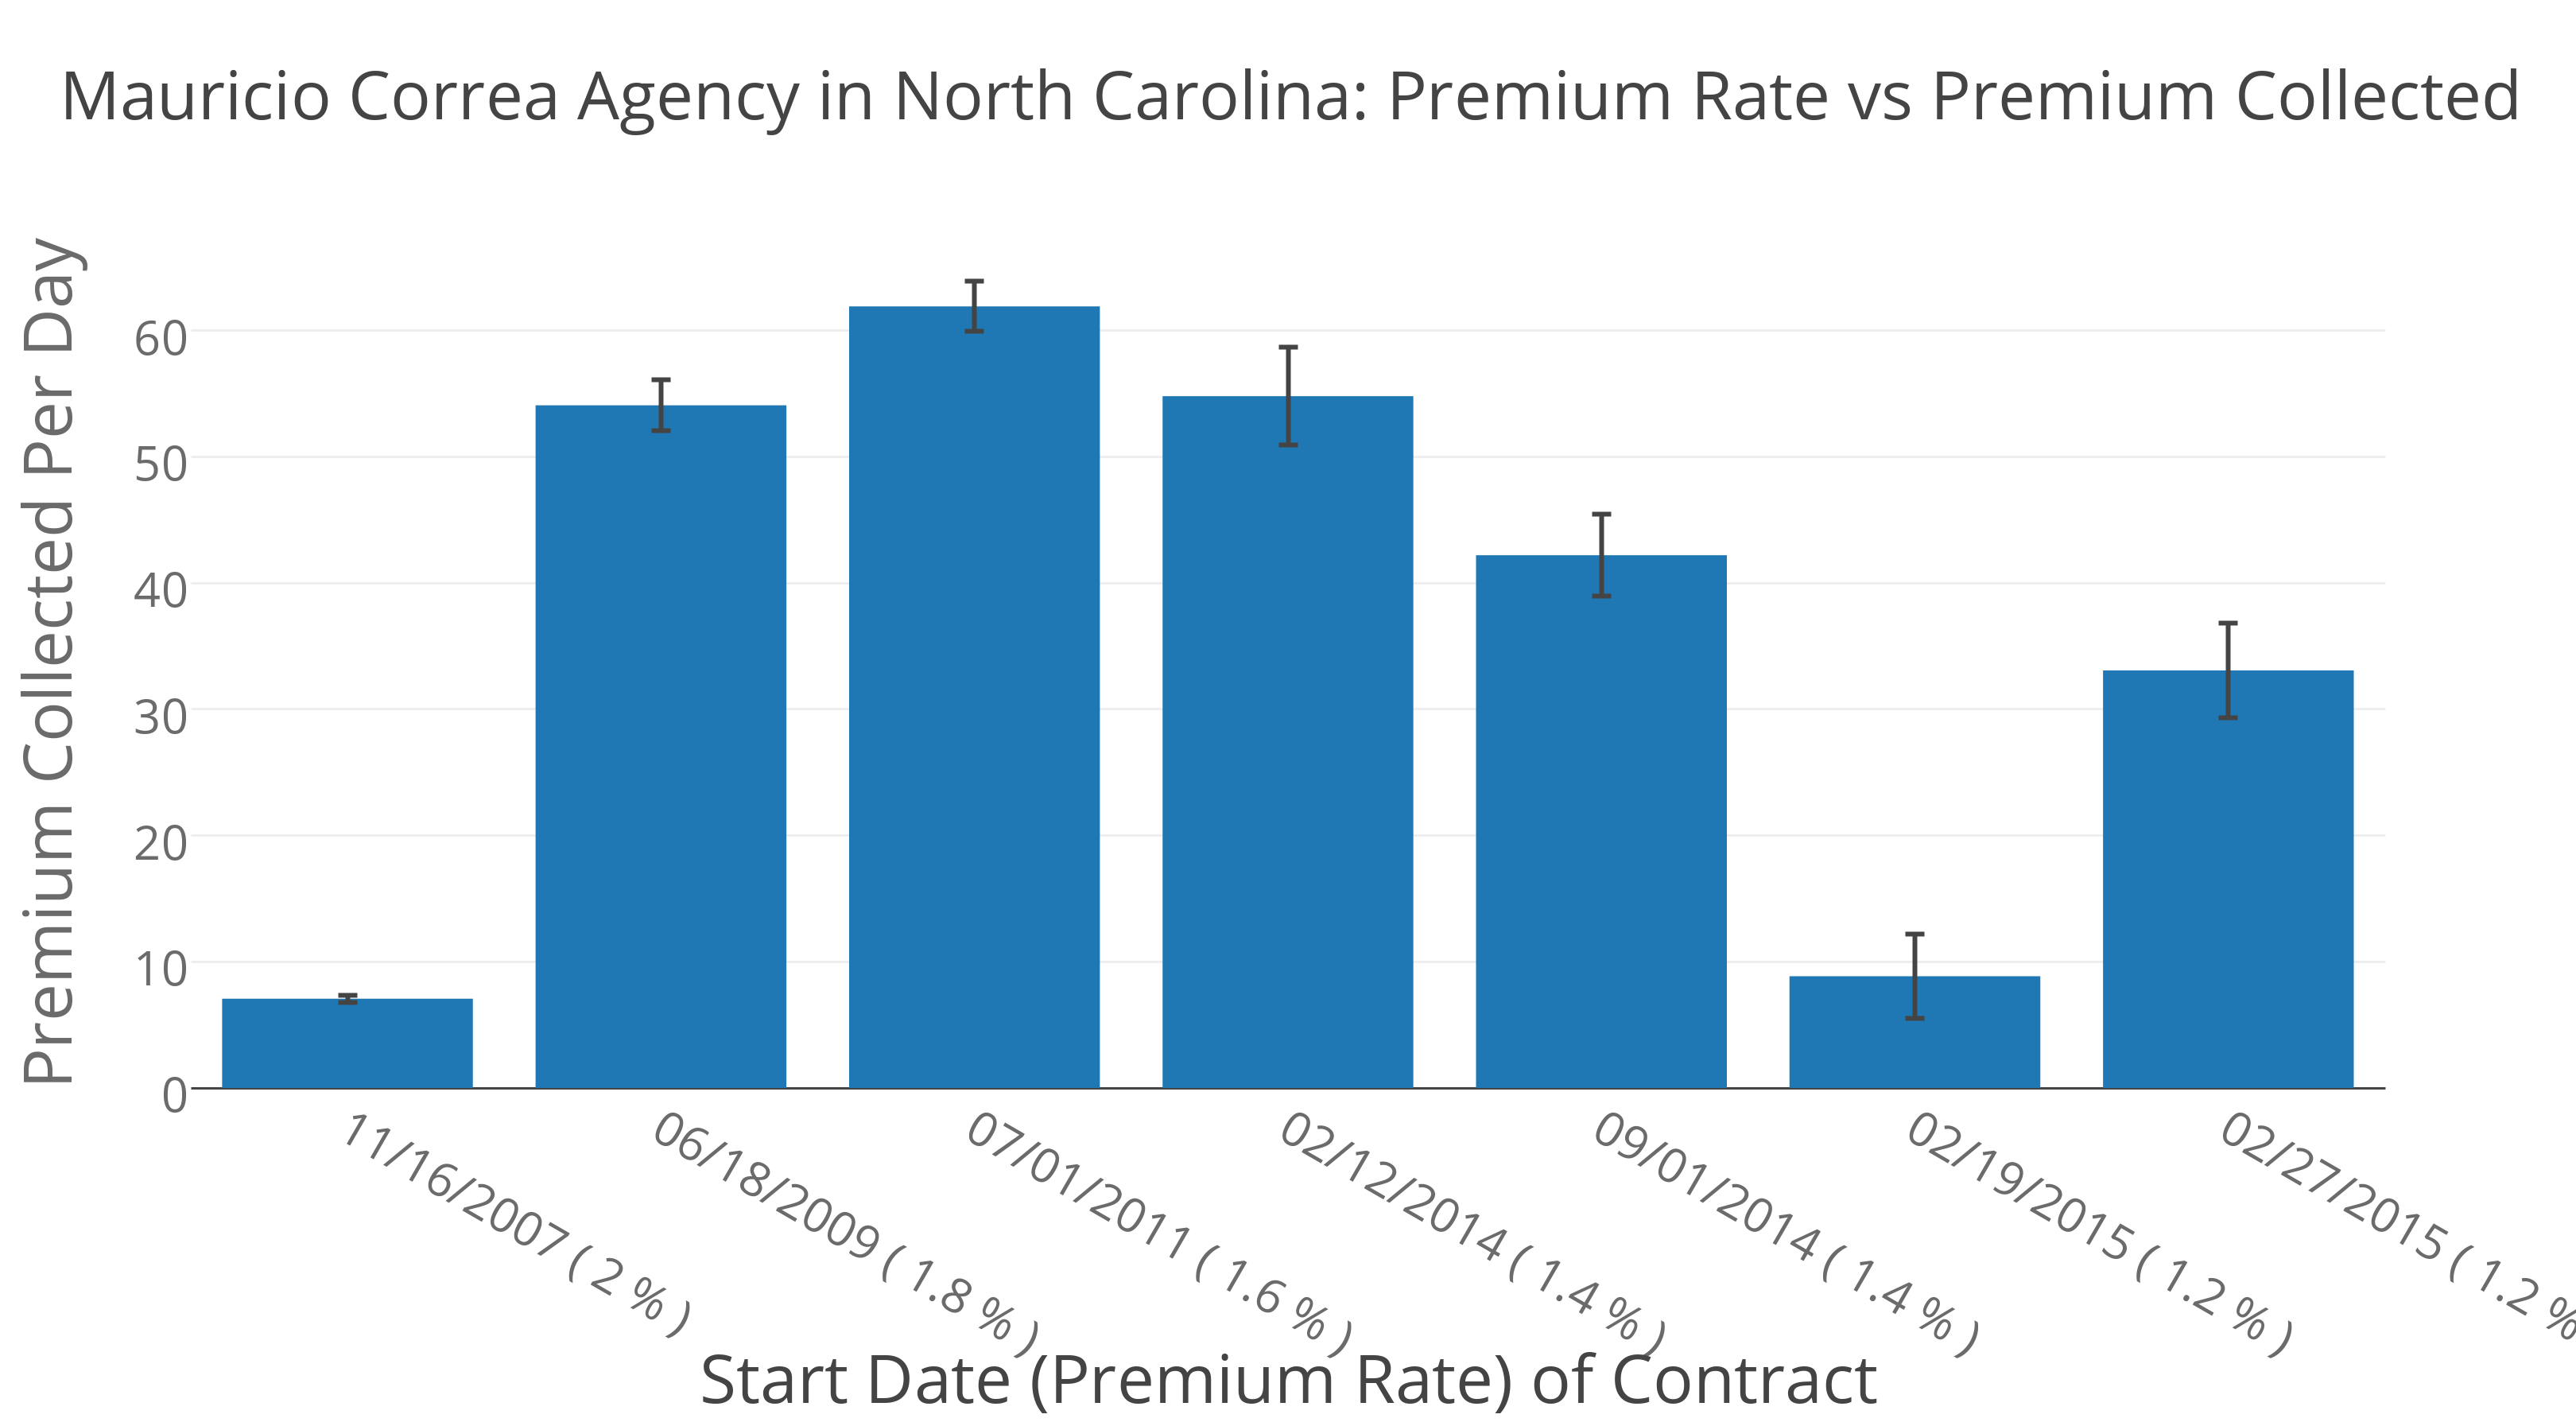
\includegraphics[width=\textwidth]{Mauricio_Correa_Agency_in_North_Carolina-_Premium_Rate_vs_Premium_Collected.png}
\end{subfigure}
\caption{Agents with varying premium rates}
\end{figure}
\end{center}
~\\

Looking at the different agencies, it becomes apparent that on average each write varying volume of penal per day.  

We can construct a linear model which relates the premium collected from agents as a function of premium rate.
Plotting these two values against each other we get: 

\begin{figure}[H]
\centering
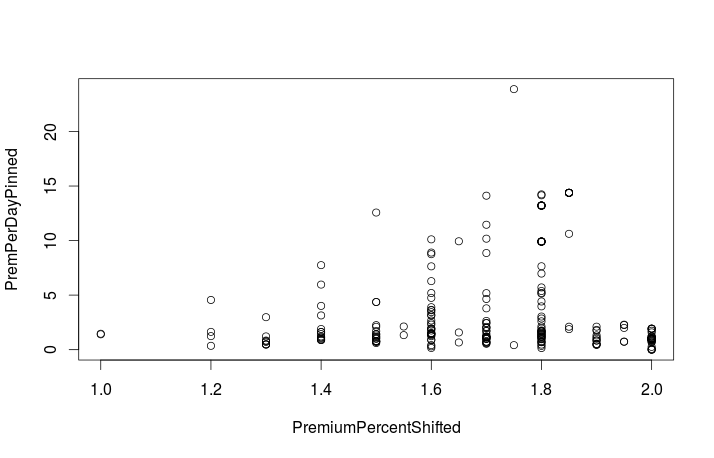
\includegraphics[width=0.45\paperwidth]{premPinnedNoLine.png}
\end{figure}



\begin{figure}[H]
\centering
\begin{BVerbatim}
Residuals:
   Min     1Q Median     3Q    Max 
-4.875 -2.978 -1.478  1.250 19.538 

Coefficients:
                      Estimate Std. Error t value Pr(>|t|)    
(Intercept)             -6.677      2.694  -2.478  0.01406 *  
PremiumPercentShifted    6.299      1.613   3.905  0.00013 ***
---
Signif. codes:  0 ‘***’ 0.001 ‘**’ 0.01 ‘*’ 0.05 ‘.’ 0.1 ‘ ’ 1

Residual standard error: 4.266 on 197 degrees of freedom
Multiple R-squared:  0.07183,Adjusted R-squared:  0.06712 
F-statistic: 15.25 on 1 and 197 DF,  p-value: 0.0001296
\end{BVerbatim}
\end{figure}


Adding another variable...\\

\begin{figure}[H]
\begin{center}
\begin{BVerbatim}
Residuals:
   Min     1Q Median     3Q    Max 
-5.875 -2.808 -1.090  1.548 20.339 

Coefficients:
                        Estimate Std. Error t value Pr(>|t|)    
(Intercept)           -4.885e+00  2.634e+00  -1.854   0.0652 .  
UnderWritingLimit      1.253e-05  3.118e-06   4.020  8.3e-05 ***
PremiumPercentShifted  4.102e+00  1.648e+00   2.489   0.0136 *  
---
Signif. codes:  0 ‘***’ 0.001 ‘**’ 0.01 ‘*’ 0.05 ‘.’ 0.1 ‘ ’ 1

Residual standard error: 4.111 on 196 degrees of freedom
Multiple R-squared:  0.1425,Adjusted R-squared:  0.1338 
F-statistic: 16.29 on 2 and 196 DF,  p-value: 2.856e-07
\end{BVerbatim}
\end{center}
\end{figure}

\begin{figure}[H]
\centering
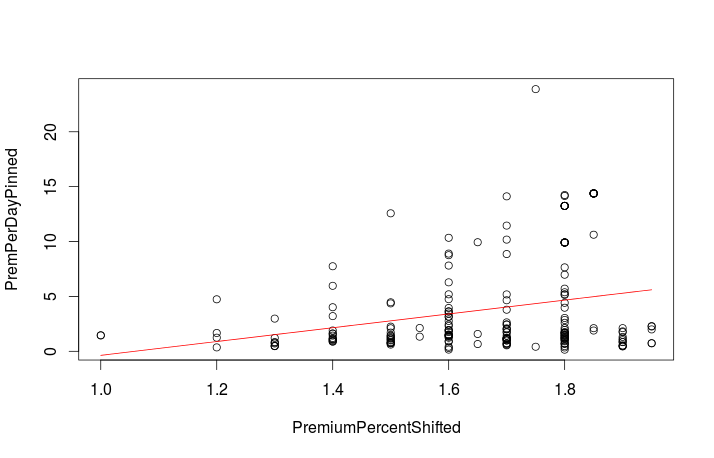
\includegraphics[width=0.45\paperwidth]{pinnedPremPerDay.png}
\end{figure}



\begin{figure}[H]
\centering
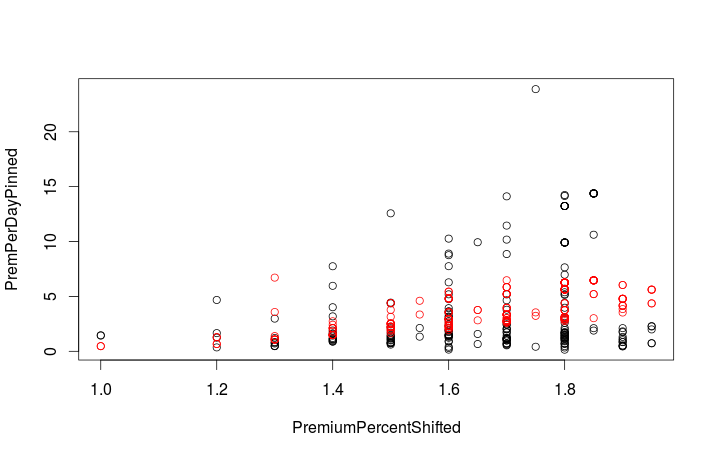
\includegraphics[width=0.45\paperwidth]{pinnedPremPerDayWithUWL.png}
\end{figure}

In some fields, it is entirely expected that your R-squared values will be low. For example, any field that attempts to predict human behavior, such as psychology, typically has R-squared values lower than 50\%. Humans are simply harder to predict than, say, physical processes.


\end{document}

